\documentclass[a4paper,dvipdfmx]{jarticle}
\usepackage{amsmath}
\usepackage{pdfpages}
\usepackage{here}
\usepackage{titlesec}
\titleformat*{\section}{\large\bfseries}
\titleformat*{\subsection}{\normalsize\bfseries}

\renewcommand{\thesection}{問題\arabic{section}}
\renewcommand{\thesubsection}{(\arabic{subsection})}


\begin{document}

\title{シミュレーション実習 中間レポート}
\author{262201018 在田 陽一}
\date{2022/05/11}
\maketitle


% 問題1
\section{}
% (1)
\subsection{}
\noindent

条件より, 棒の下半分が$y$軸と交わるためには
\begin{equation}
     y_s \leq \frac{l}{2}\sin\theta \tag{1.1}
\end{equation}
であればよい.

\noindent
$0 \leq \theta \leq \frac{\pi}{2}$, $0 \leq y_s \leq \frac{d}{2}$ より,
この範囲において変数$y_s$, $\theta$が式(1.1)を満たす確率を求めればよい.

\noindent
よって確率$p$は,
\begin{equation}
    p \sim \frac{\int^\frac{\pi}{2}_0 \frac{l}{2}\sin \theta}{\frac{\pi}{2} \cdot \frac{d}{2}} \\
     =\frac{2l}{\pi d} \tag{1.2}
\end{equation}
となる.

% (2)
\subsection{}

\noindent
式(1.2)より,
\begin{equation}
   \pi \sim  \frac{2l}{pd} \tag{1.3}
\end{equation}
と表せるので, $y_s$と$\theta$を乱数生成させることで式(1.1)と比較し,
それをもとに式(1.3)によって$\pi$を実測する.

\noindent
プログラムの実行手順としては, まずデータをbuffon.pyによって出力し,
それをproblem1.ipynbによって出力した. 
落とした棒の本数と実測した$\pi$の値の関係を図1に示す. なお, $\pi$の理論値を赤線で重ね合わせた.
\begin{figure}[H]
    \centering
    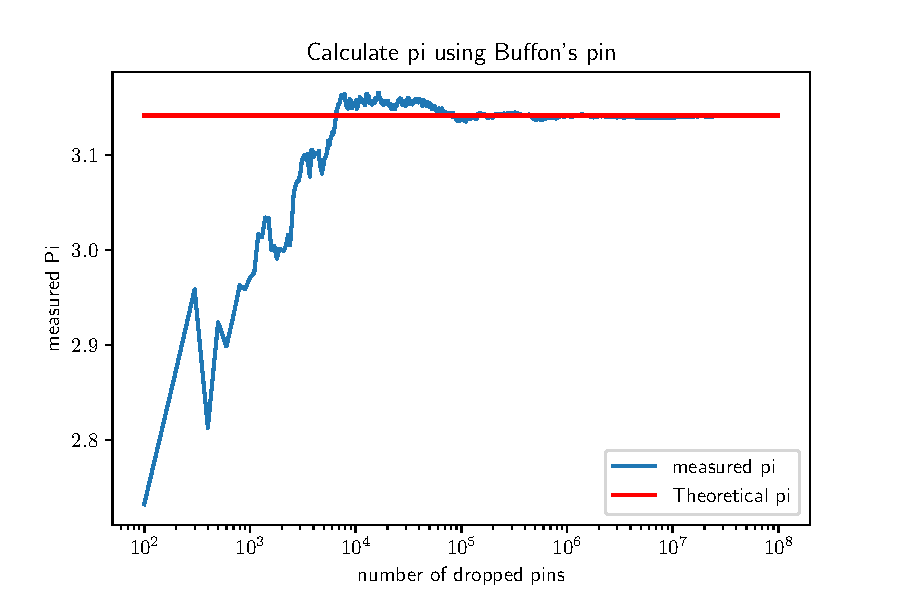
\includegraphics[scale=0.6]{./problem_1/problem1-2.pdf}
    \caption{Buffonの針による円周率の数値的見積もり}
\end{figure}

% (3)
\subsection{}
\noindent
(2)で実測した$\pi$の値と理論値の差の誤差を, 絶対値として示す. 
プログラムの実行手順としては, まずデータをbuffon.pyによって出力し,
それをproblem1.ipynbによって出力した.
誤差の絶対値と落とした棒の本数の関係を図2に示す.
ここで,$\frac{C}{\sqrt{n}}$を, $C=3.0$として重ね合わせた.
\begin{figure}[H]
    \centering
    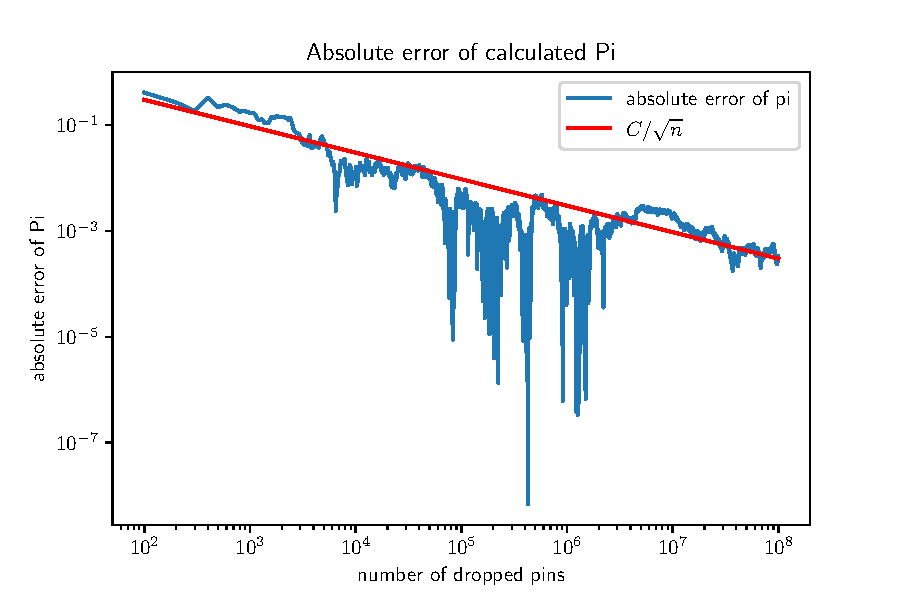
\includegraphics[scale=0.6]{./problem_1/problem1-3.pdf}
    \caption{数値的の見積もった円周率の絶対誤差}
\end{figure}

\newpage


% 問題2
\section{}
% (1)
\subsection{}

\noindent
式(1)は定数係数の二階微分方程式より, $x=e^{\lambda x}$とおいて整理すると
\begin{equation}
    m\lambda^2 + \zeta\lambda + k = 0 \tag{2.1}
\end{equation}
という特性方程式(2.1)を得る. この解は

\begin{equation}
    \lambda = \frac{-\zeta + \sqrt{\zeta^2 - 4mk}}{2} \tag{2.2}
\end{equation}
であり, ルートの中身について場合分けすると, 減衰振動, 過減衰, 臨界減衰を示す条件はそれぞれ

\begin{align*}
    \zeta & > \sqrt{4mk}   (減衰振動) \tag{2.3}\\
    \zeta & < \sqrt{4mk}   (過減衰) \tag{2.4}\\
    \zeta & = \sqrt{4mk}   (臨界減衰) \tag{2.5}\\
\end{align*}
となる.


\subsection{}

\noindent
式(1)について$x = \tilde{x}$, $t = t_0 \tilde{t}$, $\dot{x} = v = \frac{a}{t_0} \tilde{v}$
を代入して
\begin{equation}
    m \frac{a}{t_0} \dot{\tilde{v}}(\tilde{t}) = -\zeta \frac{a}{t_0} \tilde{v}(\tilde{t})
    -k a \tilde{x}(\tilde{t}) \tag{2.6}
\end{equation}
ここで

\begin{align*}
    \frac{d \tilde{v}(\tilde{t})}{dt} &= \frac{d \tilde{v}(\tilde{t})}{d \tilde{t}} \cdot \frac{d \tilde{t}}{dt} \\
    &= \frac{1}{t_0} \frac{d \tilde{v}(\tilde{t})}{d \tilde{t}} \tag{2.7}
\end{align*}
より, 式(2.6)は

\begin{equation}
    \frac{m}{t_0^2} \frac{d \tilde{v}(\tilde{t})}{d \tilde{t}} = - \frac{\zeta}{t_0} \tilde{v}(\tilde{t})
    -k \tilde{x}(\tilde{t}) \tag{2.8}
\end{equation}
と表される. 式(2.8)左辺について, 刻み幅$\Delta \tilde{t}$に関するオイラー法による離散化を実行すると

\begin{equation}
    \frac{d \tilde{v}(\tilde{t})}{d \tilde{t}} = \frac{\tilde{v}(\tilde{t} + \Delta \tilde{t}) - \tilde{v}(\tilde{t})}{\Delta \tilde{t}} 
    \tag {2.9}
\end{equation}
より, これを式(2.8)に代入して整理すると

\begin{align}
    \tilde{v}(\tilde{t} + \Delta \tilde{t}) = \left(1 - \frac{\zeta t_0 \Delta \tilde{t}}{m}\right) \tilde{v}(\tilde{t})
    - \frac{k t_0^2 \Delta \tilde{t}}{m} \tilde{x}(\tilde{t}) \tag{2.10}
\end{align}
また$\tilde{x}(\tilde{t} + \Delta \tilde{t})$について, 半陰的オイラー法に基づき

\begin{align*}
    \tilde{x}(\tilde{t} + \Delta \tilde{t}) &= \tilde{x}(\tilde{t}) + \tilde{v}(\tilde{t} + \Delta \tilde{t}) \Delta \tilde{t} \\
    &= \left(1 - \frac{k t_0^2 \Delta \tilde{t}}{m}\right) \tilde{x}(\tilde{t}) 
    + \left(1 - \frac{\zeta t_0 \Delta \tilde{t}}{m}\right) \tilde{v}(\tilde{t}) \Delta \tilde{t} \tag{2.11}
\end{align*}
以上より, 求める2項間漸化式は

\begin{subequations}
    \begin{align}
    \left\{
        \begin{aligned}
        & \tilde{v}(\tilde{t} + \Delta \tilde{t}) = \left(1 - \frac{\zeta t_0 \Delta \tilde{t}}{m}\right) \tilde{v}(\tilde{t})
        - \frac{k t_0^2 \Delta \tilde{t}}{m} \tilde{x}(\tilde{t})\\
        & \tilde{x}(\tilde{t} + \Delta \tilde{t}) = \left(1 - \frac{k t_0^2 \Delta \tilde{t}}{m}\right) \tilde{x}(\tilde{t}) 
        + \left(1 - \frac{\zeta t_0 \Delta \tilde{t}}{m}\right) \tilde{v}(\tilde{t}) \Delta \tilde{t}
        \end{aligned}
    \right. \tag{2.12}
    \end{align}
\end{subequations}
となる.

% (3)
\subsection{}

\noindent
式(2.12)について$t_d = \frac{m}{\zeta}$, $t_s = \sqrt{\frac{m}{k}}$を代入すると
\begin{subequations}
    \begin{align}
    \left\{
        \begin{aligned}
        & \tilde{v}(\tilde{t} + \Delta \tilde{t}) = \left(1 - \frac{t_0}{t_d} \Delta \tilde{t} \right) \tilde{v}(\tilde{t})
        - \left(\frac{t_0}{t_s}\right)^2 \tilde{x}(\tilde{t}) \Delta \tilde{t}\\
        & \tilde{x}(\tilde{t} + \Delta \tilde{t}) = \left[1 - \left(\frac{t_0}{t_s}\right)^2 \Delta \tilde{t} \right] \tilde{x}(\tilde{t}) 
        + \left(1 - \frac{t_0}{t_d} \Delta \tilde{t} \right) \tilde{v}(\tilde{t}) \Delta \tilde{t}
        \end{aligned}
    \right. \tag{2.13}
    \end{align}
\end{subequations}
となる.

% (4)
\subsection{}
\noindent

式(2.13)において$t_s=t_0$を代入し,さらに$\frac{t_0}{t_d}=T$とすると
\begin{subequations}
    \begin{align}
    \left\{
        \begin{aligned}
        & \tilde{v}(\tilde{t} + \Delta \tilde{t}) = \left(1 - T \Delta \tilde{t} \right) \tilde{v}(\tilde{t})
        - \tilde{x}(\tilde{t}) \Delta \tilde{t}\\
        & \tilde{x}(\tilde{t} + \Delta \tilde{t}) = (1 - \Delta \tilde{t} ) \tilde{x}(\tilde{t}) 
        + \left(1 - T \Delta \tilde{t} \right) \tilde{v}(\tilde{t}) \Delta \tilde{t}
        \end{aligned}
    \right. \tag{2.14}
    \end{align}
\end{subequations}
となる.
また, $t_d = \frac{m}{\zeta}$, $t_s = \sqrt{\frac{m}{k}}$, $t_s=t_0$を式(2.3)-(2.5)に代入することで
$\frac{t_0}{t_d}=T$とおいたとき
\begin{align*}
    T & < 2   (減衰振動) \tag{2.3}\\
    T & > 2   (過減衰) \tag{2.4}\\
    T & = 2   (臨界減衰) \tag{2.5}\\
\end{align*}
となるので, $T=0, 1, 2, 3, 4$のときの$x(t)$を図2.1にプロットした.
各$T$における$t$と$x(t)$の関係をproblem2.pyを用いて出力し, それらをproblem2.ipynb
によって1つの図にプロットした. 
ここで, $\Delta t=0.01$, $\frac{a}{t_0}=0.1$として計算し, $t$の範囲は(0,500)とした. 

\begin{figure}[H]
    \centering
    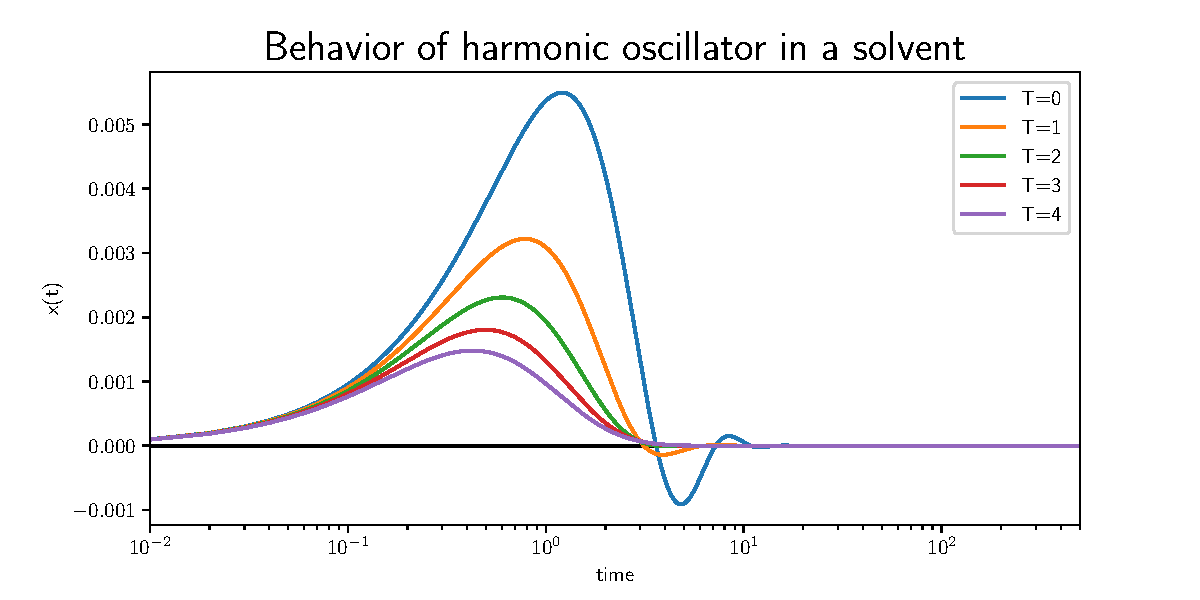
\includegraphics[scale=0.6]{./problem_2/problem2.pdf}
    \caption{調和振動子のふるまい}
\end{figure}

\newpage
\noindent
※添付ファイル \\
・buffon.py \\
・ploblem2.py \\
・ploblem1.ipynb \\
・ploblem2.ipynb

\end{document}